\documentclass{article}
\usepackage[top=1in, bottom=1in, left=1in, right=1in]{geometry}
\usepackage{graphicx}
\begin{document}

\begin{flushright}
Matt Jibson \\
EG 510 \\
HW 6
\end{flushright}

1. Find the dual of: \\
\begin{displaymath}
\begin{array}{ll}
\textrm{maximize} & z = 6x_1 - 3x_2 - 2x_3 + 5x_4 \\
\textrm{subject to} & 4x_1 + 3x_2 - 8x_3 + 7x_4 = 11 \\
& 3x_1 + 2x_2 + 7x_3 + 6x_4 \ge 23 \\
& 7x_1 + 4x_2 + 3x_3 + 2x_4 \le 22 \\
& x_1, x_2 \ge 0, x_3 \le 0, x_4\ \textrm{unrestricted}
\end{array}
\end{displaymath}

Convert to canonical form: \\
\begin{displaymath}
\begin{array}{ll}
\textrm{maximize} & z = 6x_1 - 3x_2 - 2x_3 + 5x_4 \\
\textrm{subject to} & 4x_1 + 3x_2 - 8x_3 + 7x_4 \ge 11 \\
& -4x_1 - 3x_2 + 8x_3 - 7x_4 \ge -11 \\
& 3x_1 + 2x_2 + 7x_3 + 6x_4 \ge 23 \\
& -7x_1 - 4x_2 - 3x_3 - 2x_4 \ge -22 \\
& x_1, x_2 \ge 0, x_3 \le 0, x_4\ \textrm{unrestricted}
\end{array}
\end{displaymath}

Dual is: \\
\begin{displaymath}
\begin{array}{ll}
\textrm{minimize} & w = 11y_1 -11y_2 + 23y_3 - 22y_4 \\
\textrm{subject to} & 4y_1 -4y_2 + 3y_3 - 7y_4 \le 6 \\
& 3y_1 - 3y_2 + 2y_3 - 4y_3 \le -3 \\
& -8y_1 + 8y_2 + 7y_3 - 3y_4 \ge -2 \\
& 7y_1 - 7y_2 + 6y_3 -2y_4 = 5 \\
& y_1, y_2, y_3, y_4 \ge 0
\end{array}
\end{displaymath}

2. Find dual of: \\
\begin{displaymath}
\begin{array}{ll}
\textrm{maximize} & z = -x_1 - x_2 \\
\textrm{subject to} & -x_1 + x_2 \ge 1 \\
& 2x_1 - x_2 \le 2 \\
& x_1, x_2 \ge 0
\end{array}
\end{displaymath}

Graph: \\
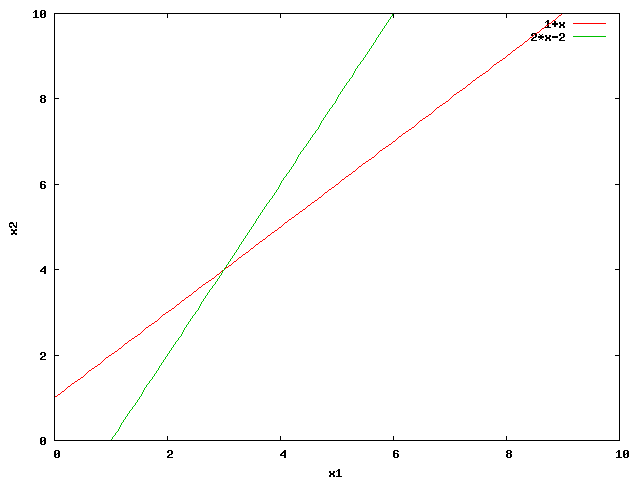
\includegraphics[width=0.5\linewidth]{2b} \\
At $\mathbf{x} = (0, 1)^T$, $z$ is maximized at $-1$. \\

Dual is: \\
\begin{displaymath}
\begin{array}{ll}
\textrm{minimize} & w = y_1 + 2y_2 \\
\textrm{subject to} & -y_1 + 2y_2 \ge -1 \\
& y_1 - y_2 \ge -1 \\
& y_1 \le 0, y_2 \ge 0
\end{array}
\end{displaymath}

Graph: \\
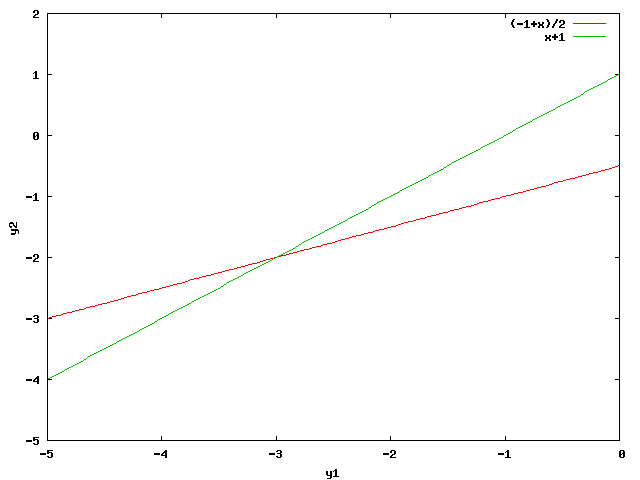
\includegraphics[width=0.5\linewidth]{2a} \\
At $\mathbf{y} = (-1, 0)^T$, $w$ is minimized at $-1$. Strong duality is verified: both optima are $-1$. \\

3. Find dual of: \\
\begin{displaymath}
\begin{array}{ll}
\textrm{minimize} & z = 2x_1 + 9x_2 + 3x_3 \\
\textrm{subject to} & -2x_1 + 2x_2 + x_3 \ge 1 \\
& x_1 + 4x_2 - x_3 \ge 1 \\
& x_1, x_2, x_3 \ge 0
\end{array}
\end{displaymath}

Dual is: \\
\begin{displaymath}
\begin{array}{ll}
\textrm{maximize} & w = y_1 + y_2 \\
\textrm{subject to} & -2y_1 + y_2 \le 2 \\
& 2y_1 + 4y_2 \le 9 \\
& y_2 - y_2 \le 3 \\
& y_1, y_2 \ge 0
\end{array}
\end{displaymath}

Graph: \\
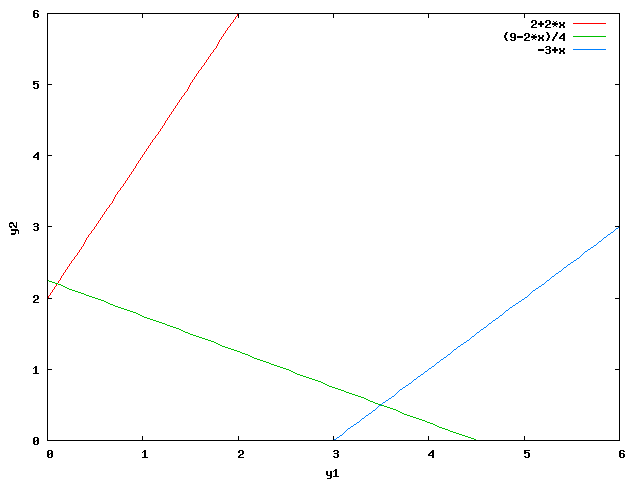
\includegraphics[width=0.4\linewidth]{3a} \\
At $\mathbf{y} = (4.5, 0)^T$, $w$ is maximized at $4.5$. \\

\newpage

In the dual the first two constraints are binding. Using complementary slackness, the last one constraint in the primal must be binding. Graphically solving: \\
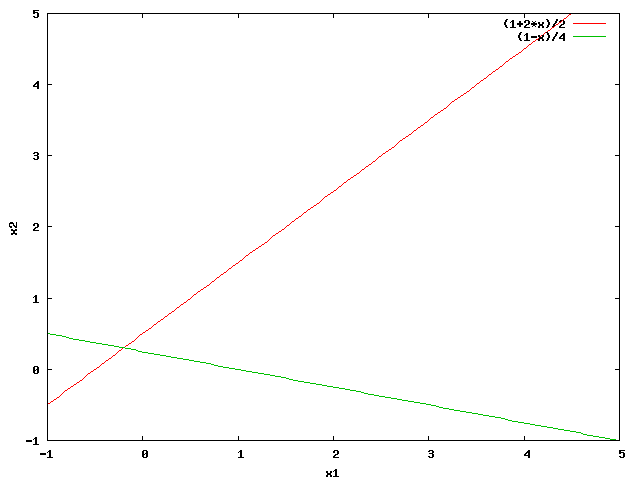
\includegraphics[width=0.4\linewidth]{3b} \\
At $\mathbf{x} = (0, 0.5, 0)^T$, $z$ is minimized at $4.5$. \\

4. Find dual of: \\
\begin{displaymath}
\begin{array}{ll}
\textrm{minimize} & z = 2x_1 + 9x_2 + 3x_3 \\
\textrm{subject to} & \frac{3}{7}x_1 + 2x_2 + x_3 \ge 1 \\
& x_1 + 4x_2 - x_3 \ge 1 \\
& x_1, x_2, x_3 \ge 0
\end{array}
\end{displaymath}

Dual is: \\
\begin{displaymath}
\begin{array}{ll}
\textrm{maximize} & w = y_1 + y_2 \\
\textrm{subject to} & \frac{3}{7}y_1 + y_2 \le 2 \\
& 2y_1 + 4y_2 \le 9 \\
& y_2 - y_2 \le 3 \\
& y_1, y_2 \ge 0
\end{array}
\end{displaymath}

Graph: \\
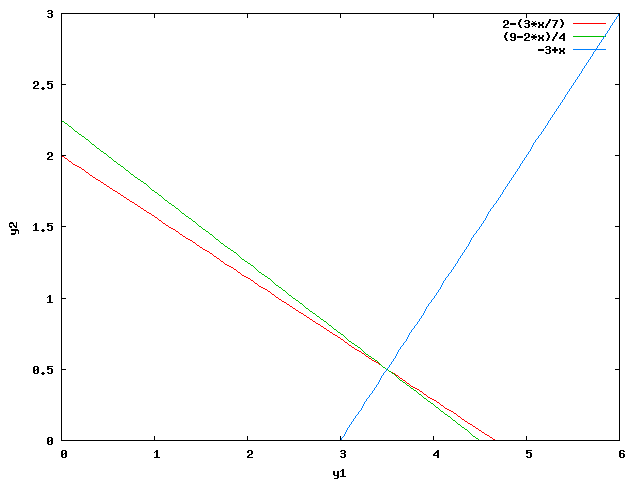
\includegraphics[width=0.4\linewidth]{4a} \\
At $\mathbf{y} = (4.5, 0)^T$, $w$ is maximized at $4.5$. \\

\newpage

In the dual the first two constraints are binding. Using complementary slackness, the last one constraint in the primal must be binding. Graphically solving: \\
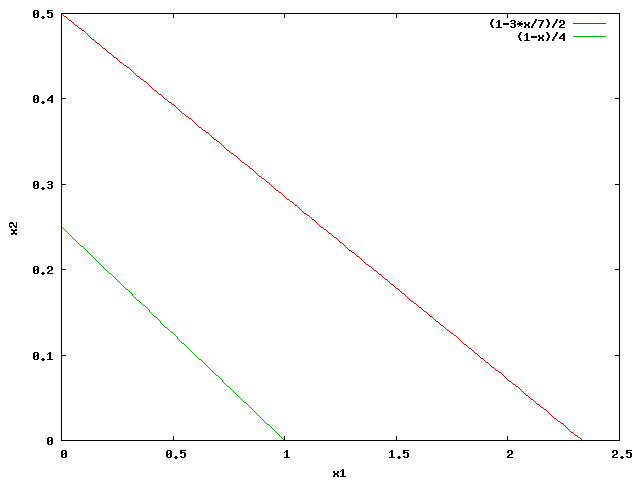
\includegraphics[width=0.4\linewidth]{4b} \\
At $\mathbf{x} = (0, 0.5, 0)^T$, $z$ is minimized at $4.5$. (Apparently I did something wrong as I don't think this is the right answer.)\\

\end{document}
